

\chapter{Verificarea formală a implementării algoritmului}

În următoarea schemă voi exemplifica modul în care se apelează metodele, funcțiile și lemele pentru a demonstra faptul 
că implementarea algoritmului greedy rezolva problema bancnotelor și produce soluția optimă.\par
    \vspace{1cm}
\setcounter{figure}{0}
    \begin{figure}[h]
        \centering
          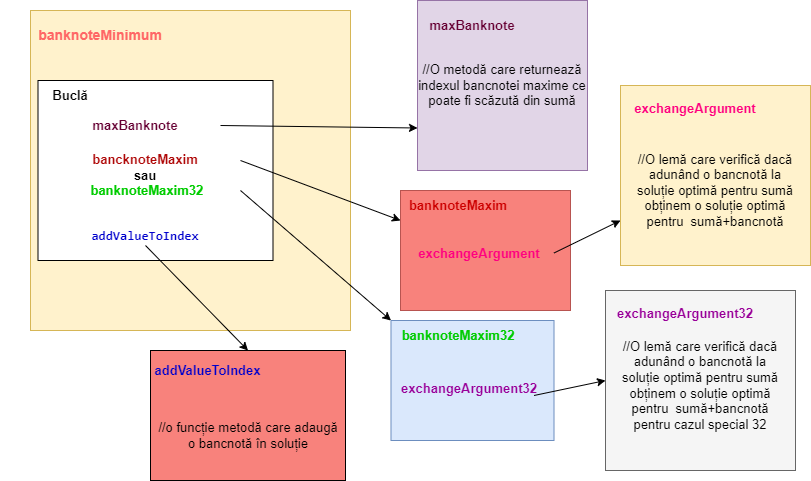
\includegraphics[width=1.0\textwidth]{verification_schema}
      \end{figure} \par
Figura 1: O schemă explicativă a verificării.


  \section{Metoda banknoteMinimum}
    Metoda banknoteMinimum este metoda principală folosită pentru a returna soluția optimă pentru o sumă dată ca 
    input.\par
    Această metodă are ca precondiții faptul că suma este pozitivă, iar ca postcondiții avem cele 3 predicate menționate 
    anterior care asigură optimalitatea unei soluții.\par
    Metoda folosește o buclă, în care, la fiecare iterație, se adaugă cea mai mare bancnotă mai mică decât sum construind soluția.\par
    În primă fază calculează bancnota cea mai mare ce poate fi dată ca rest, cu ajutorul funcției maxBanknote, detaliată în 3.3 și funcției 
    power, care calculează ridicarea la putere.\par
    Dificultatea principală este de a demonstra că proprietatea de optimalitate se menține pe parcursul buclei.\par
    Invarianții prezenți în while (liniile 12,13,14) au rolul de a menține proprietatea de optimalitate 
    pe parcursul construirii soluției, astfel că la orice pas soluția este optimă pentru $suma-rest$.\par
    Primul invariant are rolul de a se asigura că pe parcursul construirii soluției nu avem de dat rest negativ.\par
    Al doilea invariant, explicat în subcapitolul 2.1, are rolul de a se asigura că soluția construită se menține optimă, aici ne ajuta funcția 
    metodă care garantează că dacă adunăm o anumită bancnotă la soluție, aceasta încă este validă.\par
    Al treilea invariant,pentru care voi da exemplu de cod mai jos, nu poate fi verificat de Dafny așa că acest invariant trebuie demonstrat cu ajutorul lemei banknoteMaxim sau banknoteMaxim32(detaliate în capitolul 3.4, respectiv 3.6), 
    în funcție de bancnota aleasă.\par
    La final bancnota optimă este adaugată în sumă cu ajutorul funcției addValueToIndex, detaliată în subcapitolul 3.2, iar din rest se scade valoarea bancnotei adaugată în sumă.
    \begin{lstlisting}
    method banknoteMinimum(sum: int) returns(solution: seq <int> )
        requires sum >= 0
        ensures isValidSolution(solution)
        ensures isSolution(solution, sum)
        ensures isOptimalSolution(solution, sum) 
    {
        var rest:= sum;
        solution:= [0, 0, 0, 0, 0, 0];
        var index:= 0;
        assert isOptimalSolution(solution, sum - rest);
        while (0 < rest)
            invariant 0 <= rest <= sum
            invariant isValidSolution(solution)
            invariant addOptimRestEqualsOptimSum(rest, sum, solution)
            decreases rest 
        {
            index:= maxBanknote(rest);
            var banknote:= power(2, index);
            if (index != 5) 
            {
                banknoteMaxim(rest, sum, solution, index);
            } 
            else 
            {
                banknoteMaxim32(rest, sum, solution);
            }
            solution:= addValueToIndex(solution,1,index);
            rest:= rest - banknote;
        }
    }
    \end{lstlisting}

$\bullet$ \textbf{predicatul addOptimRestEqualsOptimSum}: Acest predicat(de la linia 14) are rolul de a verifica dacă o soluție pentru suma $x$ 
adunată cu o soluție optimă pentru suma $y$ are ca rezultat o soluție optimă pentru $x+y$. Acest lucru ne ajută să verificăm 
optimalitatea unei soluții fără să fie necesară optimalitatea ambelor soluții ce o formează.\par
Scopul acestor predicate este de a asigura că secvența ce reprezintă datele de ieșire respectă toate condițiile necesare
pentru a fi considerată soluție optimă.

\section{Funcția addValueToIndex}
Funcția addValueToIndex este folosită pentru a adăuga unui element din soluție o valoare, folosindu-ne de index-ul acestuia.\par
Este utilă pentru construirea soluțiilor.\par
Aceasta are drept precondiții pentru modificarea corectă a sumei faptul că index-ul trebuie să fie în codomeniu, soluția să fie validă și
faptul că valoarea adaugată plus valoarea inițială a elementului din secvență nu reprezintă un număr negativ.\par
Postcondițiile acestei funcții ne asigură faptul că avem o soluție validă în urma adaugării și faptul că valoarea sumei pe care 
o reprezintă soluția a crescut cu valoarea la care ne așteptam.\par
\begin{lstlisting}
function method addValueToIndex(solution: seq<int>, value: int, index: int): seq<int>
  requires 0 <= index <= 5
  requires isValidSolution(solution)
  requires solution[index] + value >= 0
  ensures isValidSolution(solution)
  ensures solutionElementsSum(solution) + value*power(2, index) == solutionElementsSum(solution[index:=solution[index]+value])
{
  solution[index:= solution[index] + value]
}
\end{lstlisting}


    \section{Metoda maxBanknote}
    Metoda maxBanknote este folosită pentru a returna un index cu proprietatea: \par
     $bancnota_{index} <= rest < bancnota_{index + 1}$  .\par
     Avem postcondițiile următoare: indexul să se afle în codomeniu-ul secvenței, bancnota corespunzătoare indexului să fie mai mică decât suma,
     și un index nu poate fi mai mare decât a fost calculat fără depăși suma.
     Aceste postcondiții au fost necesare pentru a demonstra faptul că indexul returnat este întradevăr corespunzător celei
     mai mari bancnote care poate fi dată rest pentru sum.
    \begin{lstlisting}
      method maxBanknote(sum: int) returns(index: int)
        requires sum > 0
        ensures 0 <= index <= 5
        ensures 0 <= power(2, index) <= sum
        ensures(index != 5 && power(2, index + 1) > sum) || index == 5 
      {
        index:= 5;
        if (power(2, index) > sum) 
        {
          assert power(2, index + 1) > sum;
          while (power(2, index) > sum && index > 0)
            invariant power(2, index + 1) > sum 
            {
              index:= index - 1;
              assert power(2, index + 1) > sum;
            }
        } 
          else 
        {
          assert index == 5;
        }
      }
    \end{lstlisting}


    \section{Lema banknoteMaxim}
    Lema banknoteMaxim este tratată diferit de lema banknoteMaxim32 deoarece avem o bancnotă nemărginită superior, bancnota 32,
    care trebuie tratată separat.
    Lema banknoteMaxim este folosită pentru a demonstra păstrarea faptului că dacă adăugam o bancnotă în soluția pe care o 
    construim, în continuare suma acestei soluții cu soluția optimă pentru $ rest - bancnota$ va produce soluția 
    optimă pentru suma întreagă.\par
    Pentru a demonstra că o soluție este optimă, încercăm să găsim o soluție cu cost mai mic, dacă nu reușim, atunci 
    știm că soluția găsită este optimă~\cite{kozen1993optimal}.
    Avem nevoie să știm că dacă în soluția curentă, optimă pentru $ rest - bancnota$  
    adaugăm bancnota, aceasta devine optimă pentru $rest$. Acest lucru este demonstrat cu ajutorul lemei exchangeArgument.
    Aceste lemme au nevoie ca indexul să se afle în codomeniu și să fie ales conform metodei maxBanknote, soluția calculată până 
    în prezent să fie validă și să respecte predicatul addOptimRestEqualsOptimSum, așadar acestea sunt precondițiile.
    Această metodă asigură că predicatul addOptimRestEqualsOptimSum este valid pentru $rest $ dacă scădem bancnota aleasă din rest, 
    de aceea este postcondiție.
    \begin{lstlisting}
    lemma banknoteMaxim(rest: int, sum: int, finalSolution: seq <int> , index: int)
        requires 0 <= index <= 4
        requires power(2, index) <= rest < power(2, index + 1)
        requires isValidSolution(finalSolution)
        requires addOptimRestEqualsOptimSum(rest, sum, finalSolution)
        ensures addOptimRestEqualsOptimSum(rest - power(2, index), sum, finalSolution[index:= finalSolution[index] + 1]) 
    {
        var banknote:= power(2, index);
        forall currentSolution | isValidSolution(currentSolution) && isOptimalSolution(currentSolution, rest - banknote)
            ensures isOptimalSolution(solutionsSum(solutionsSum(currentSolution, finalSolution), [0, 0, 0, 0, 0, 0][index:= 1]), sum) 
        {
            assert isSolution(currentSolution[index:= currentSolution[index] + 1], rest);
            exchangeArgument(rest, currentSolution, index);
        }
        assert forall currentSolution::isValidSolution(currentSolution) && isOptimalSolution(currentSolution, rest - banknote) ==> isOptimalSolution(solutionsSum(solutionsSum(currentSolution, finalSolution), [0, 0, 0, 0, 0, 0][index:= 1]), sum);
    }
    \end{lstlisting}


    \section{Lema banknoteMaxim32}
    Lema banknoteMaxim32 este folosită pentru a demonstra invariantul addOptimRestEqualsOptimSum.\par
    Lema este similară cu banknoteMaxim, doar că este specifică bancnotei nemărginite, 32.
    Avem nevoie să știm că dacă în soluția curentă, optimă pentru $ rest - 32$  
    adaugăm bancnota, aceasta devine optimă pentru $rest$. Acest lucru este demonstrat cu ajutorul 
    lemei exchangeArgument32, detaliat in subcapitolul   ???.
    Aceste lemme au nevoie ca indexul să se afle în codomeniu și să fie ales conform metodei maxBanknote, 
    soluția calculată până în prezent să fie validă și să respecte predicatul addOptimRestEqualsOptimSum, 
    așadar acestea sunt precondițiile.
    Această metodă se asigură că predicatul addOptimRestEqualsOptimSum este valid pentru $rest $ dacă scădem bancnota 32 din rest, 
    de aceea este postcondiție.

\begin{lstlisting}
lemma banknoteMaxim32(rest: int, sum: int, finalSolution: seq < int > )
  requires rest >= 32
  requires isValidSolution(finalSolution)
  requires addOptimRestEqualsOptimSum(rest, sum, finalSolution)
  ensures addOptimRestEqualsOptimSum(rest - 32, sum, solutionsSum(finalSolution, [0, 0, 0, 0, 0, 1])) 
{
  forall currentSolution | isValidSolution(currentSolution) && isSolution(currentSolution, rest - 32)
    ensures isSolution(solutionsSum(solutionsSum(finalSolution, currentSolution), [0, 0, 0, 0, 0, 1]), sum) 
  {
    assert isSolution(solutionsSum(currentSolution, [0, 0, 0, 0, 0, 1]), rest);
  }

  forall currentSolution | isValidSolution(currentSolution) && isOptimalSolution(currentSolution, rest - 32)
    ensures isOptimalSolution(solutionsSum(solutionsSum(finalSolution, currentSolution), [0, 0, 0, 0, 0, 1]), sum)
  {
    forall someSolution | isValidSolution(someSolution) && isSolution(someSolution, sum)
      ensures cost(someSolution) >= cost(solutionsSum(solutionsSum(finalSolution, currentSolution), [0, 0, 0, 0, 0, 1])) 
    {
      exchangeArgument32(rest, sum,  currentSolution);
    }
  }
}
\end{lstlisting}

    \section{Lema exchangeArgument}
    Lema exchangeArgument este tratată diferit de lema exchangeArgument32 deoarece avem o bancnotă nemărginită superior, bancnota 32,
    care trebuie tratată separat.\par
    Lema exchangeArgument este o lemă tipică algoritmilor greedy care se bazează pe ideea că modificând progresiv 
    dintr-o soluție produsă de orice alt algoritm într-o soluție produsă de algoritmul greedy, dacă folosim un mod 
    care să nu înrăutățească calitatea soluției, atunci costul soluției produse este cel puțin la fel de mic ca 
    cea a oricărei alte soluții, acesta fiind argumentul de schimb.\par
    Presupunem că avem o soluție optimă oarecare și arătăm că poate fi transformată într-o soluție optimă care corespunde 
    celei construite cu metoda greedy.\par
    În lema exchangeArgument presupunem că soluția nu este optimă dacă adaugăm bancnota aleasă și ajungem la o contradicție.
    Știm că soluția e optimă pentru $rest - bancnota$, dar nu pentru rest, dacă adaugăm bancnota(linia 13).\par
    Considerăm că există o altă soluție optimă pentru rest, numită optimalSolution(linia 15).\par
    Următoarea verificare este specifică cazurilor $1,2,4,8,16$.\par
    Verificăm în presupusa soluție pentru rest că nu avem bancnota în soluție deja(linia 17), altfel dacă din acea presupusă 
    solutie am scădea bancnota, atunci am avea un cost mai mic decât costul soluției noastre care e optimă pentru 
    $rest - bancnota$ din precondiție, deci avem o contradicție.\par
    Ulterior, demonstrăm că invariantul, explicat mai jos, de la linia 19, se menține pe parcursul unei bucle.\par
    Nu există două bancnote de aceeași valoare în soluție, mai mici de 32.\par
    În acest mod știm că soluția presupusă nu poate fi optimă, deoarece, dacă respectă proprietatea
    suma produsă de aceasta nu poate fi egală cu rest. \par
    Deoarece :\par
    $\bullet \sum_{k=0}^{index-1} 2^{k} = 2^{index}-1 $\par
    $\bullet rest > = 2^{index} $ \par
    Deci presupusa soluție pentru rest nu poate fi egală decât cu cel mult $rest- 1$(linia 45), astfel nu poate fi soluție optimă și se ajunge la o contradicție. 
    Precondițiile și postcondițiile necesare pentru acestor lemme sunt aceleași ca în lemma banknoteMaxim.\par
    
    \begin{lstlisting}
lemma exchangeArgument(rest: int, currentSolution: seq <int> , index: int)
    requires 0 <= index <= 4
    requires power(2, index) <= rest < power(2, index + 1)
    requires isValidSolution(currentSolution)
    requires isOptimalSolution(currentSolution, rest - power(2, index))
    ensures isOptimalSolution(currentSolution[index:= currentSolution[index] + 1], rest) 
{
    var banknote:= power(2, index);
    var solution:= currentSolution[index:= currentSolution[index] + 1];
    assert isValidSolution(solution);
    assert isSolution(solution, rest);
    var i:= index;
    if (!isOptimalSolution(solution, rest)) 
    {
        var optimalSolution:| isValidSolution(optimalSolution) && isSolution(optimalSolution, rest) &&
            isOptimalSolution(optimalSolution, rest) && cost(optimalSolution) < cost(solution);
        if (optimalSolution[index] -1 >= 0) 
        {
            var betterSolution:= addValueToIndex(optimalSolution,-1,index);
            assert isSolution(betterSolution, rest - banknote);
            assert cost(betterSolution) == cost(optimalSolution) - 1;
            assert cost(optimalSolution) - 1 < cost(currentSolution);
            assert false;
        } 
        else 
        {
            while (0 < i)
            invariant 0 <= i <= index
            invariant forall x::index >= x >= i ==> optimalSolution[x] <= 1 
            {
            i:= i - 1;
            assert isOptimalSolution(optimalSolution, rest);
            if (optimalSolution[i] > 1) 
            {
                var optimalSolution' := optimalSolution[i:=optimalSolution[i]-2];
                optimalSolution' := optimalSolution' [i + 1:= optimalSolution'[i+1]+1];
                assert isSolution(optimalSolution', rest);
                assert cost(optimalSolution') == cost(optimalSolution) - 1;
                assert cost(optimalSolution') < cost(optimalSolution);
                assert false;
            }
            }
            assert solutionElementsSum(optimalSolution) <= banknote - 1;
            assert rest >= banknote; 
            assert solutionElementsSum(optimalSolution) <= rest - 1; 
            assert isOptimalSolution(optimalSolution, rest); 
            assert false;
        }
    }
}
    \end{lstlisting}
        
$\bullet$ \textbf{invariant}:Acest invariant(de la linia 29) se asigură că 
nu avem în soluția optimă mai mult de o bancnotă de valoarea 1, 2, 4, 8 sau 16, deoarece aparițiile multiple ale acestora pot fi
înlocuite cu o bancnotă superioară pentru optimalitate(2 bancnote de valoare 1 au costul mai mare decât o bancnotă de valoare 2).\par
\begin{lstlisting}
    invariant forall index :: 4 >= index >= i ==> optimalSolution[index] <= 1
\end{lstlisting}

\section{Lema exchangeArgument32}

Presupunem că avem o soluție optimă oarecare și arătăm că poate fi transformată într-o soluție optimă care corespunde 
celei construite cu metoda greedy.\par
În lema exchangeArgument32 presupunem că soluția nu este optimă dacă adaugăm bancnota 32 și ajungem la o contradicție.
Știm că soluția e optimă pentru $rest - 32$, dar nu pentru rest, dacă adaugăm bancnota(linia 10).\par
Considerăm că există o altă soluție optimă pentru rest, numită optimalSolution(linia 15).\par
Demonstrăm că invariantul, explicat anterior, de la linia 25, se menține pe parcursul buclei.\par
Nu există două bancnote de aceeași valoare în soluție, mai mici de 32.\par
În acest mod știm că soluția presupusă nu poate fi optimă, deoarece, dacă respectă proprietatea
suma produsă de aceasta nu poate fi egală cu rest. \par
$\bullet \sum_{k=0}^{index-1} 2^{k} = 2^{index}-1 $\par
$\bullet rest > = 2^{index} $ \par
Deci presupusa soluție pentru rest nu poate fi egală decât cu cel mult $rest- 1$(linia 38), astfel nu poate fi soluție optimă și se ajunge la o contradicție. 
Precondițiile și postcondițiile necesare pentru acestor lemme sunt aceleași ca în lema banknoteMaxim32.\par

\begin{lstlisting}
    
lemma exchangeArgument32(rest: int, sum: int,  optimalSolution: seq < int > )
    requires 32 <= rest
    requires isValidSolution(optimalSolution)
    requires isOptimalSolution(optimalSolution, rest - 32)
    ensures isOptimalSolution(optimalSolution[5:= optimalSolution[5] + 1], rest) 
{
    var solution:= optimalSolution[5:= optimalSolution[5] + 1];
    var i:= 4;
    if (!isOptimalSolution(solution, rest)) 
    {
        if (optimalSolution[i] > 1) 
        {
            var solution:= optimalSolution[i:= optimalSolution[i] - 2];
            solution:= solution[i + 1:= solution[i + 1] + 1];
            assert isSolution(solution, rest - 32);
            assert cost(solution) == cost(optimalSolution) - 1;
            assert cost(optimalSolution) - 1 < cost(solution);
            assert false;
        } 
        else
        {
            while (0 < i)
                invariant 0 <= i <= 4
                invariant forall index::4 >= index >= i ==> optimalSolution[index] <= 1 
            {
            i:= i - 1;
            if (optimalSolution[i] > 1) 
                {
                    var solution:= optimalSolution[i:= optimalSolution[i] - 2];
                    solution:= solution[i + 1:= solution[i + 1] + 1];
                    assert isSolution(solution, rest - 32);
                    assert cost(solution) == cost(optimalSolution) - 1;
                    assert cost(optimalSolution) - 1 < cost(solution);
                    assert false;
                }
            }
            assert solutionElementsSum(optimalSolution) <= rest - 1;
            assert isOptimalSolution(solution, rest);
            assert false;
        }
    }
}
\end{lstlisting}
